\section{MR image reconstruction}\label{sec:IMrec}

Different pulse sequences and certain physiological properties that can be exploited with certain pulse sequences, have been laid out in the previous sections. This section aims to describe how the corresponding echo signals are reconstructed as a MR image.

Following the Lamour frequency \eqref{eq:lamour}, the main magnetic field causes all hydrogen nuclei to precess with the same frequency. Without any specification of spatial localization a MRI of a human body would consist of a single number. To prevent this, separate coils in the x, y and z directions are introduced. These coils can be adjusted in position, and thus produce gradient magnetic fields with a varying strength depending on position. According to the Lamour frequency the nuclei will precess with different frequencies when in a magnetic field with varying strength. The gradients can be turned on in combination to create any direction in space. These varying frequencies can be exploited to separate parts of the anatomy and ultimately illustrate a desired area. As mentioned, the nuclei only exchange energy efficiently if the frequency of energy, or RF pulse, matches the precession rate. Thus, by altering the magnetic field along the body in one direction, z-direction for the sake of the example, the nuclei will have slightly different precession rates, and the RF pulse will only efficiently affect a desired slice of the nuclei.
The nuclei of that slice now precess at the same rate. To get an image with a spatial resolution, the voxels that make out the image needs to be discriminated between. By turning on the gradient of the x-direction the lines in the y-direction are now encoded with a particular frequency. This gradient functions as a frequency encoding gradient, and is illustrated in \figref{fig:back:gradient}. \cite{Bharath2008} \\
 \begin{figure}[H]                 
	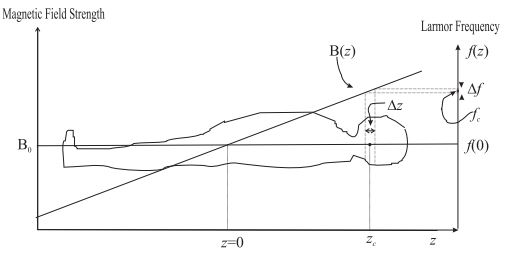
\includegraphics[width=.7\textwidth]{figures/aBackground/gradient}  
	\caption{The position of the slice is specified through the direction of the frequency encoding gradient ($B(z)$) and though the central frequency of the emitted RF pulse ($f_c$). The thickness of the slice is dependent on the steepness slope of $B(z)$, and on the bandwith of the emitted RF pulse $(\delta f)$. \cite{Bharath2008}}
	\label{fig:back:gradient} 
\end{figure}
Turning the y-gradient on and quickly off, will de-phase the nuclei while still remaining the same frequency as before. This gradient functions as a phase encoding gradient. When comparing two locations approximately one voxel apart in the x-direction, then based on the amount of gradient strength difference, there will be a certain amount of change in phase between the spins spread across that distance. The farther away from isocenter, where the magnetic field strength is $B_0$, the higher the change in phase will be. This notion is used to assign the correct spatial location of each voxel, when reconstructing the FID signals into an image. This phase encoding procedure is done in different gradient strengths in iterations to assign unique phases to the nuclei in the both directions. One iteration of a certain strength of the phase encoding gradient followed by a measurement is performed at a time. The only change per iteration is the phase encoding gradient strength. These iterations are then series of measurements acquired at different points in time, where each entry of the slice then represent a certain signal intensity. This time domain measurement is referred to at the raw data. \cite{Bharath2008}\\
The next step is to Fourier Transform (FT) the raw data, which will yield frequency information to the acquired signal intensities. This step gives a summation of the signal intensities at the different frequencies produced by the frequency encoding gradient. This is called the k-space, as the k-numbers of a signal describes its relative orientation and frequency. The k-space image contains the contrast in the center and the resolution in the periphery, as there is low or no phase encoding at the center and increasing towards the periphery, giving more brightness in the center and dimmer tones in the periphery. To allocate the voxels in correct spatial localization an inverse 2D discrete FT is performed on the k-space image. This provides the desired image of the anatomy slice. \cite{Bharath2008} \Figref{fig:back:kspace} shows the acquired signal in k-space and the reconstructed image after the Fourier Transform. 

\begin{figure}[H]                 
	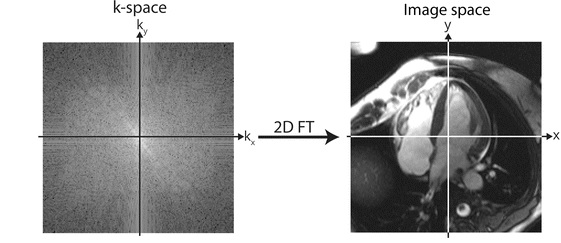
\includegraphics[width=.8\textwidth]{figures/aBackground/k_space}  
	\caption{A depiction of the acquired signal represented in k-space and the resulting reconstructed image after the inverse 2D Fourier Transform \cite{Syed2015}.}
	\label{fig:back:kspace} 
\end{figure}